En el ámbito de las matemáticas y las ciencias de la computación, se emplea el término \emph{``grafo''} (del griego \emph{``grafos''} que significa \emph{``dibujo''} o \emph{``imagen''}) para referirse a un conjunto de objetos llamados \emph{``vértices''} o \emph{``nodos''}, los cuales están unidos por enlaces conocidos como \emph{``aristas''} o \emph{``arcos''}. Estas conexiones representan las relaciones binarias que existen entre los elementos de un conjunto, y son objeto de estudio de la teoría de grafos.

En la Figura \ref{fig:grafo1} se muestra un ejemplo de grafo.

\begin{figure}[H]
\centering
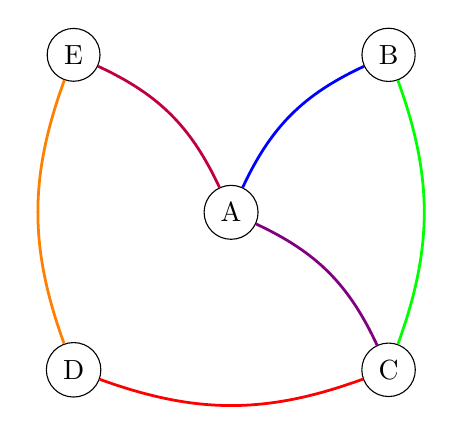
\begin{tikzpicture}

% Posiciones fijas de los nodos
\node[circle, draw=black, fill=white] (A) at (0,0) {A};
\node[circle, draw=black, fill=white] (B) at (2,2) {B};
\node[circle, draw=black, fill=white] (C) at (2,-2) {C};
\node[circle, draw=black, fill=white] (D) at (-2,-2) {D};
\node[circle, draw=black, fill=white] (E) at (-2,2) {E};

% Arcos aleatorios
\draw[-, blue, line width=1pt] (A) to[bend left=20] (B);
\draw[-, green, line width=1pt] (B) to[bend left=20] (C);
\draw[-, red, line width=1pt] (C) to[bend left=20] (D);
\draw[-, orange, line width=1pt] (D) to[bend left=20] (E);
\draw[-, purple, line width=1pt] (E) to[bend left=20] (A);
\draw[-, violet, line width=1pt] (A) to[bend left=20] (C);

\end{tikzpicture}
\caption{Ejemplo de grafo con $5$ nodos.}
\label{fig:grafo1}
\end{figure}

Matemáticamente, un grafo $G = (V,E)$ es una tupla de vértices $V$ y aristas $E$ que relacionan dichos vértices. Denominaremos  \emph{orden} del grafo al número de vértices del mismo ($|V|$). Por supuesto, siempre tendremos que $V \neq \emptyset$.

Asimismo, se denomina \emph{grafo dirigido} o \emph{digrafo} a aquellos grafos cuyas aristas tengan un sentido definido. Por el contrario, las aristas de los grafos no dirigidos representan relaciones simétricas.

En la Figura \ref{fig:grafo2} se muestra un ejemplo de grafo dirigido.

\begin{figure}[H]
\centering
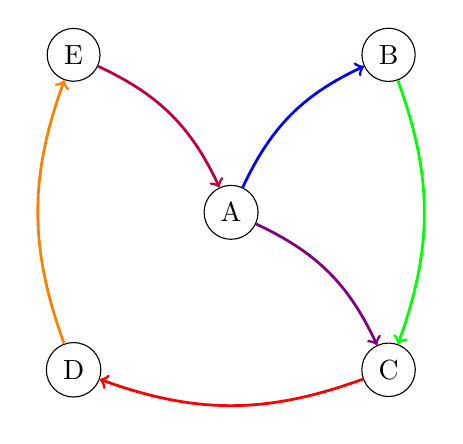
\begin{tikzpicture}

% Posiciones fijas de los nodos
\node[circle, draw=black, fill=white] (A) at (0,0) {A};
\node[circle, draw=black, fill=white] (B) at (2,2) {B};
\node[circle, draw=black, fill=white] (C) at (2,-2) {C};
\node[circle, draw=black, fill=white] (D) at (-2,-2) {D};
\node[circle, draw=black, fill=white] (E) at (-2,2) {E};

% Arcos aleatorios
\draw[->, blue, line width=1pt] (A) to[bend left=20] (B);
\draw[->, green, line width=1pt] (B) to[bend left=20] (C);
\draw[->, red, line width=1pt] (C) to[bend left=20] (D);
\draw[->, orange, line width=1pt] (D) to[bend left=20] (E);
\draw[->, purple, line width=1pt] (E) to[bend left=20] (A);
\draw[->, violet, line width=1pt] (A) to[bend left=20] (C);

\end{tikzpicture}
\caption{Ejemplo de grafo dirigido con $5$ nodos.}
\label{fig:grafo2}
\end{figure}

Mientras que en un grafo no dirigido se tiene que $E \subseteq \{x \in \mathcal{P}(V) : |x| = 2\}$ (es decir, $E$ es un conjunto de pares no ordenados de elementos de $V$), cuando el grafo es dirigido se tiene que $E$ es un conjunto de pares ordenados $(i,j) \in V \times V$.
 
No obstante, en este trabajo fin de grado nos serán de gran utilidad los llamados \emph{grafos dirigidos acíclicos} o \emph{DAG} (\emph{Directed Acyclic Graphs}, en inglés) que no son más que grafos dirigidos desprovistos de ciclos.

En la Figura \ref{fig:grafo3} se muestra un ejemplo de grafo acíclico dirigido. Por el contrario, el grafo que se muestra en la figura \ref{fig:grafo2} no es acíclico (tiene ciclos, por ejemplo, el $A$-$C$-$D$-$E$).

\begin{figure}[H]
\centering
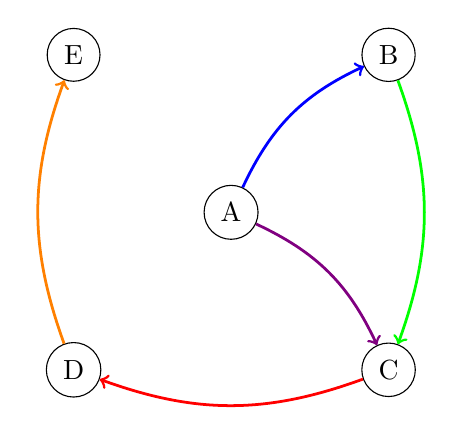
\begin{tikzpicture}

% Posiciones fijas de los nodos
\node[circle, draw=black, fill=white] (A) at (0,0) {A};
\node[circle, draw=black, fill=white] (B) at (2,2) {B};
\node[circle, draw=black, fill=white] (C) at (2,-2) {C};
\node[circle, draw=black, fill=white] (D) at (-2,-2) {D};
\node[circle, draw=black, fill=white] (E) at (-2,2) {E};

% Arcos aleatorios
\draw[->, blue, line width=1pt] (A) to[bend left=20] (B);
\draw[->, green, line width=1pt] (B) to[bend left=20] (C);
\draw[->, red, line width=1pt] (C) to[bend left=20] (D);
\draw[->, orange, line width=1pt] (D) to[bend left=20] (E);
\draw[->, violet, line width=1pt] (A) to[bend left=20] (C);

\end{tikzpicture}
\caption{Ejemplo de grafo acíclico dirigido con $5$ nodos.}
\label{fig:grafo3}
\end{figure}